\documentclass{tufte-handout}

\title{Building support for improving transport: \\ Nine strategies \& a framework}

\author{James Reynolds, PTRG, Monash University}

%\date{28 March 2010} % without \date command, current date is supplied

%\geometry{showframe} % display margins for debugging page layout

\usepackage{graphicx} % allow embedded images
  \setkeys{Gin}{width=\linewidth,totalheight=\textheight,keepaspectratio}
  \graphicspath{{graphics/}} % set of paths to search for images
\usepackage{amsmath}  % extended mathematics
\usepackage{booktabs} % book-quality tables
\usepackage{units}    % non-stacked fractions and better unit spacing
\usepackage{multicol} % multiple column layout facilities
\usepackage{lipsum}   % filler text
\usepackage{fancyvrb} % extended verbatim environments
\usepackage{natbib}
  \fvset{fontsize=\normalsize}% default font size for fancy-verbatim environments

% Standardize command font styles and environments
\newcommand{\doccmd}[1]{\texttt{\textbackslash#1}}% command name -- adds backslash automatically
\newcommand{\docopt}[1]{\ensuremath{\langle}\textrm{\textit{#1}}\ensuremath{\rangle}}% optional command argument
\newcommand{\docarg}[1]{\textrm{\textit{#1}}}% (required) command argument
\newcommand{\docenv}[1]{\textsf{#1}}% environment name
\newcommand{\docpkg}[1]{\texttt{#1}}% package name
\newcommand{\doccls}[1]{\texttt{#1}}% document class name
\newcommand{\docclsopt}[1]{\texttt{#1}}% document class option name
\newenvironment{docspec}{\begin{quote}\noindent}{\end{quote}}% command specification environment

\begin{document}

\maketitle% this prints the handout title, author, and date


\begin{marginfigure}%
  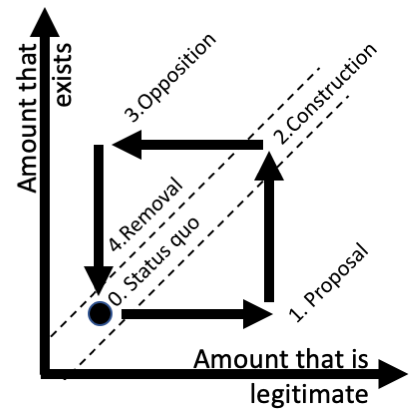
\includegraphics[width=\linewidth]{Framework_and_progression}
  \caption{Legitimacy framework and a simple progression}
  \label{fig:Legitimacy_framework}
\end{marginfigure}
  


\begin{abstract}
\noindent
Why is improving transport so hard? How can bus or bike lanes, pedestrian malls and other beneficial (but potentially unpopular or controversial) measures be successfully implemented? This handout outlines a new framework (Figure \ref{fig:Legitimacy_framework}) and nine pragmatic strategies
%\footnote{Building legitimacy before implementation through (A1) technical enquiry, (A2) transport planning or (A3) public processes; avoiding impacts through (B1) grade separation, (B2) new capacity, or (B3) subservience; and building legitimacy through implementation using (C1) bottom-up and incremental implementation, (C2) pop-ups, and/or (C3) trials.}%
that may help you improve transport in the real-world of politics, NIMBYism and other non-technical challenges.
\end{abstract}

\smallcaps{Legitimacy} comes in many forms\footnote{Normative, sociological, through trust, through reasonableness, through unconditional duty, through public consent, or associated with conditional normative support.}, and what is considered legitimate might vary by arena\footnote{For example, installing a bus or bike lane might be the 'best' option according to engineers and planners, yet considered unreasonable amongst drivers or local business owners.} and/or change over time. Figure \ref{fig:Legitimacy_framework} shows a new framework for understanding legitimacy and implementation, which emerged from a recent PhD project\cite{Reynolds:2020aa}, and a simple progression in which an improvement is proposed and built, but then opposed and removed. Other progressions (Figure \ref{fig:Failure_or_compromise}) might lead to rejection of a proposal entirely or a compromise, such as if a High Occupancy Vehicle (HOV) lane is provided despite a bus lane warrant being met. 

\begin{marginfigure}%
  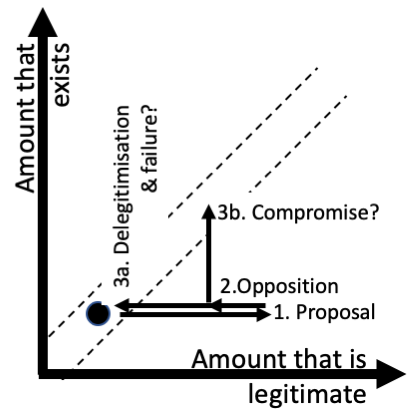
\includegraphics[width=\linewidth]{Failure_or_compromise}
  \caption{Failure or compromise}
  \label{fig:Failure_or_compromise}
\end{marginfigure}



\newthought{Nine pragmatic strategies} for legitimising implementation emerged from the case research described in this handout. The research looked at successful and not-as-successful implements of pedestrian malls, bicycle lanes and transit priority measures in Curitiba, Zürich, Boston, Toronto and Melbourne.  The first three strategies involve \textbf{building legitimacy BEFORE implementation}. This might take the form of (A1) \textbf{Technical Reporting}, but in a manner that aims to built support beyond just engineers and planners. Figure \ref{fig:Toronto_dashboard} provides an example, with monthly dashboards during the King Street Transit Pilot contrasting transit performance improvements with impacts on other road users and changes to economic activity. 

\begin{marginfigure}%
  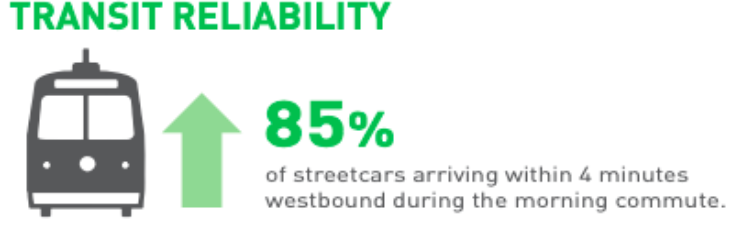
\includegraphics[width=\linewidth]{Toronto_dashboard_1}
   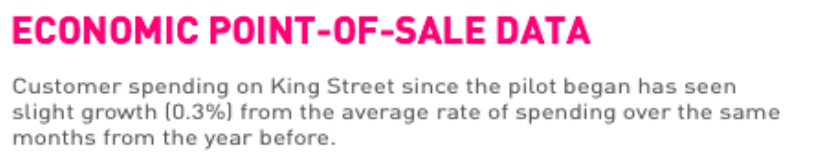
\includegraphics[width=\linewidth]{Toronto_dashboard_4}
  \caption{City of Toronto monthly dashboard during King Street Pilot (excerpt), see thesis p.274}
  \label{fig:Toronto_dashboard}
\end{marginfigure}

A (A2) \textbf{Transport Plan} can help build legitimacy, but the research findings suggest that vision-based plans might be more likely to succeed. Curitiba's famous Bus Rapid Transit (BRT) network provides an example, having been supported by a plan for transport and land-use to develop along linear 'Structural Axes' (regardless of mode). Similarly the Citizens' Transit Priority Initiative in Zürich called for buses and trams to "travel along their lanes or tracks virtually as fast as is technically possible"\cite{Nash:2001ab}. These contrast to Melbourne's Stud Road, where bus lanes were installed in accordance with a specific objective\footnote{Building bus lanes, rather than a vision of higher bus speeds and reliability}, but later partially removed after a change of government. (A3) \textbf{Public Processes} might also be used. Again Zürich provides an example, with a public ballot narrowly approving the Citizens' Transit Priority Initiative (51-49). Direct democracy deciding transport policy appears rare, but the research found cases where council meetings, environmental assessment hearings and other public processes (including court hearings) appear to have legitimised implementation.  



\begin{marginfigure}%
  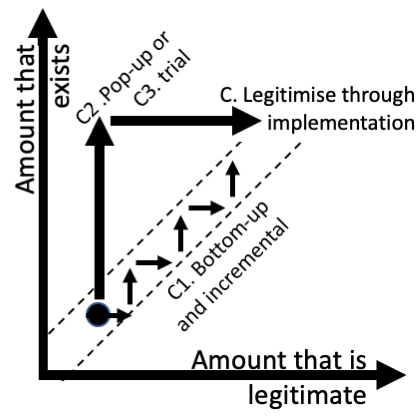
\includegraphics[width=\linewidth]{Figure4}
  \caption{Building legitimacy through implementation}
  \label{fig:FIgure4}
\end{marginfigure}

\newthought{But, why not simply} \textbf{AVOID IMPACTING} those who might oppose implementation?  This approach was successful for the Eglinton Crosstown LRT in Toronto, some of which is (B1) \textbf{Grade-separated} so as not to impact traffic. In the context of Mayor Rob Ford's declaration that "the war on the car is over"\cite{Kalinowski:2010ab} putting transit underground (even though very expensive) may have been the only way to prioritise transit in a narrow road corridor. Similarly,  the Stud Road bus lanes were only removed where they had been converted from a traffic lane. Parts where they had been built as (B2) \textbf{Additional Capacity} through road widening remain in place to this day.  (B3) \textbf{Subservient priority} similarly seeks to limit opposition  by doing everything that can be done to help transit, but without impacting motorists. This is the genesis of Curibita's famous tubular bus stops\footnote{First introduced on new 'direct bus' services running in mixed traffic, rather than along the busways. These decreased dwell time, so as to increase frequency and therefore capacity, but did not impact on other road users.} and helps explains the retention of hook turns in Clarendon Street in Melbourne\footnote{Unlike far side stops, which were removed after opposition from local businesses, hook turns improved conditions for transit and could be provided without on-street parking removal.}. 

\newthought{Legitimacy} \textbf{THROUGH} \smallcaps{implementation} relates to the idea that “if they had a chance to actually see it, everyone would love it” (attributed to Curitiba's Mayor, Jamie Lerner\cite{McKibben:2007aa}). With \textbf{C1. bottom-up and incremental implementation} successive small changes are made, seeking to build on initial successes. The gradual addition of tram separation kerbing in central Melbourne over recent decades provides an example\footnote{Sometimes during track renewal works.   In other cases tram priority measures have been included as part of works to make stops level-boarding accessible.}. (C2) \textbf{Pop-ups} and \textbf{C3. Trials} provide other ways in which people can see what changes might look like in the real-world, without having to commit to permanence first.  For Jamie Lerner, it might help that he had the support of the military dictatorship ruling Brazil at the time his team converted central Curitiba into a pop-up pedestrian mall, but the guerrilla bike lanes of Seattle\cite{Fucoloro:2013aa} and pop-up bus lanes in Boston and elsewhere\cite{Transportation-Studies:2019aa} provide examples within democracies. At the least, as shown by Clarendon Street tram priority trial\cite{Silkstone:2005aa}, temporary implementations might indicate which measures actually are legitimate enough to be kept.

Standards, technical analysis and other planning and engineering activity might help us determine what is technically appropriate. The nine strategies, sometimes individually but often together, have previously helped to build legitimacy for improving transport in Curitiba, Zürich, Boston, Toronto, Melbourne and elsewhere. These, and other research outcomes and examples discussed in the PhD thesis, may help you make progress in the real world of institutions, public support (or lack of it), politics and other non-technical factors. 

\nobibliography{implementation_transit_priority_handout}
\bibliographystyle{plainnat}



\end{document}
